%++++++++++++++++++++++++++++++++++++++++
% Don't modify this section unless you know what you're doing!
\documentclass[a4,11pt]{article}
\usepackage{pgfplots}
\usepackage{tabularx} % extra features for tabular environment
\usepackage{amsmath}  % improve math presentation
\usepackage{graphicx} % takes care of graphic including machinery
\usepackage[margin=1in,letterpaper]{geometry} % decreases margins
\usepackage{cite} % takes care of citations
\usepackage[final]{hyperref} % adds hyper links inside the generated pdf file
%\usepackage{gensymb}
\hypersetup{
  colorlinks=true,       % false: boxed links; true: colored links
  linkcolor=blue,        % color of internal links
  citecolor=blue,        % color of links to bibliography
  filecolor=magenta,     % color of file links
  urlcolor=blue         
}
\usepackage{float}
\makeatletter
\newcommand*{\rom}[1]{\expandafter\@slowromancap\romannumeral #1@}
\makeatother
% ++++++++++++++++++++++++++++++++++++++++

\begin{document}
\title{NTC Thermistor Sensor}
\author{Catherine Beryl Basson, Piotr Chromi\'nski}
\date{13 December 2016}
\maketitle
\twocolumn
\section{Introduction}

The NTC thermistors display non-linear resistance characteristics with temperature. The resistance of an NTC will decrease at the temperature increases. This behaviour is related to it's constant value $B$. This phenomenon allows for use of an NTC thermistor as a temperature sensor. In the discussed experiments a Vishay NTCLE100E3 thermistor was used, with $B=3977^{\circ}K$.

\section{Theory}
\subsection{Expected Output}
The output of thermistor is said to be non-linear, for the NTCLE100E3 it can be described with equation for expected intermediate temperatures, taken from the NTC's datasheet:
\begin{equation}
  \label{eq:datasheet}
  R_T(T)=R_{ref}\cdot e^{A+\frac{B}{T}+\frac{C}{T^2}+\frac{D}{T^3}}
\end{equation}
where $A$, $B$, $C$, and $D$ are constant values which are dependent on the thermistor; $R_{ref}$ is the resistance at a reference temperature---for the thermistor used in the experiment (Brown, Black, and Orange bands) it is $10000\Omega$,and the constant values:
\begin{center}
  \begin{tabular}{ll}
    \hline 
    $R_{ref}$  &  $10000\Omega$  \\
    $A$  &  $-14.6337$  \\
    $B$\footnotemark  &  $4791.842$  \\
    $C$  &  $-115334$  \\
    $D$  &  $-3.730535\cdot10^6$  \\
    \hline
  \end{tabular}
  \footnotetext{Note that this value is different to the $\beta$ ``$B$'' value of a thermistor, constants from this table should only be used in combination with eqation~\ref{eq:datasheet}}
\end{center}
Since, the temperature $T$ in the equation~\ref{eq:datasheet} is in $^\circ K$ for measurements in $^\circ C$ conversion is required:
\begin{equation}
  \label{eq:ctok}
T_K=T_C+273.15^\circ
\end{equation}
The Siemens Handout describes how the output can be linearised in a range by use of a prallel resistor. The equation for the value of such resistor is:
\begin{equation}
  \label{eq:siemens}
R_p=R_{T_{ctr}}\cdot\frac{B-T_{ctr}}{B+2\cdot T_{ctr}}
\end{equation}
where $R_{T_{ctr}}$ and $T_{ctr}$ are thermistor's resistance and temperature at the center of the temperature range, and $B$ is the $B$ ($\beta$) value of the thermistor. From this equation an ideal straight line equation for the linear sensor model can be found by calculating Output for $I_{min}$ and $I_{max}$, then sensitivity $K$ is
$$K=\frac{O(I_{max})-O(I_{min})}{I_{max}-I_{min}}$$
and y-intercept is
\begin{equation}
  \label{eq:intercept}
  a=O(I_{min})-KI_{min}
\end{equation}
the following experiments all measurements are compared against the linear model
\begin{equation}
  O(I)=KI+a
\end{equation}
\begin{figure}[H]
  \label{fig:parallel}
  \centering
  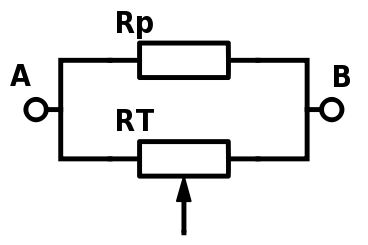
\includegraphics[width=0.75\columnwidth]{parallel.png}
  \caption{
    Parallel circuit
  }
\end{figure}
The expected output $R_{AB}(T)$ for a linearised thermistor setup shown in Fig.\ref{fig:parallel} can be derived from a basic equation for resistor:
\begin{equation}
  \label{eq:Rab}
  R_{AB}(T)=\frac{R_p\cdot R_T(T)}{R_p+R_T(T)}
\end{equation}
\section{Experiments}
Two experiments were conducted. First, to determine characteristics of the non-linear response of the NTC:\@ resistance-temperature R-T and temperature-resistance T-R, maximum non-linearity $\hat N$ as \% of $f.s.d$ (full scale deflection); response of a system linearised by a parallel resistor. Second, to find the time constant $\tau$ of the measurement system. Raw data from all measurements is presented in the Appendix.
\subsection{R-T Characteristics}

To measure the R-T and T-R characteristics the resistance was measured with an AMPROBE AM-510-EUR multimeter, and recorded over temperature range 90--45$^{\circ}C$. This was achieved by measuring the temperature of water in a cup, which was cooled from$~100^{\circ}$ to$~45^{\circ}$.

To determine the parallel resistor value $R_{T_{ctr}}$ was recorded at $T_{ctr}=72.5^{\circ}C$ and calculated using the eqation.
\subsection{Time Constant}
\section{Results}
Here, the data from each part the experiments are analysed and discussed. Important graphs, equations, and tables are shown directly in these subsections. Complete calculated data will be put into tables, graphs that can be seen in the Appendix.
\subsection{R-T Characteristics}
\subsubsection{Non-Linear}
The equation for the ideal straight line for input range 45--90$^\circ$ was found using the equation from the datasheet
$$K=\frac{R_T(90)-R_T(45)}{90-45}=\frac{0.915443-4.37181}{90-45}=-0.07681$$aprox
$$a=R_T(45)-KI_{min}=4.37181+0.07681\cdot45=7.828$$
The R-T expected output with combined data from all non-linear measurement runs is shown in the following figure:
\begin{figure}[H]
  \centering
  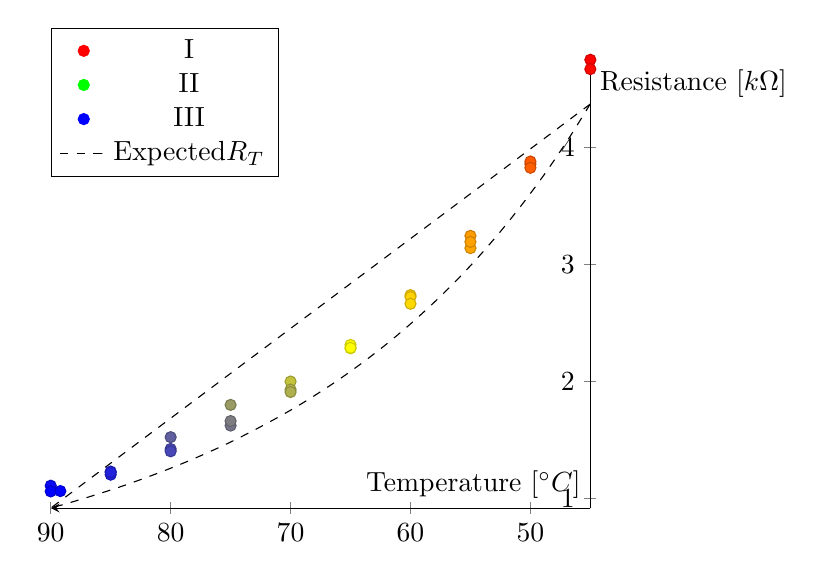
\begin{tikzpicture}
    \begin{axis}[
      axis lines=middle,
      x dir=reverse,
      legend style={
        at={(axis cs:90,3.75)},
        anchor=south west},
      xlabel=Temperature \lbrack$^{\circ}C$\rbrack,
      ylabel=Resistance \lbrack$k\Omega$\rbrack,
      ]
      \addplot[scatter,
      only marks,
      color=red,
      mark=*
      ] coordinates {
        (90, 1.107)
        (85, 1.228)
        (80, 1.522)
        (75, 1.798)
        (70, 1.998)
        (65, 2.311)
        (60, 2.737)
        (55, 3.244)
        (50, 3.858)
        (45, 4.75)
      };
      \addlegendentry{\rom{1}}
      \addplot[scatter,
      only marks,
      color=green,
      mark=*,
      ] coordinates {
        (90, 1.058)
        (85, 1.201)
        (80, 1.421)
        (75, 1.621)
        (70, 1.929)
        (65, 2.282)
        (60, 2.721)
        (55, 3.139)
        (50, 3.88)
        (45, 4.67)
      };
      \addlegendentry{\rom{2}}
      \addplot[scatter,
      only marks,
      color=blue,
      mark=*,
      ] coordinates {
        (89.2, 1.061)
        (85, 1.221)
        (80, 1.401)
        (75, 1.66)
        (70, 1.908)
        (65, 2.286)
        (60, 2.663)
        (55, 3.192)
        (50, 3.826)
      };
      \addlegendentry{\rom{3}}
      \addplot[smooth, black, dashed][domain=45:90]{10*exp(-14.6337+(4791.842/(x+273.15)+(-115334/((x+273.15)^2))+((-3.730535*1000000)/((x+273.15)^3)))};
      \addlegendentry{Expected$R_T$}
      \addplot[smooth, black, dashed][domain=45:90]{-0.0768081*x+7.8281};

    \end{axis}
  \end{tikzpicture}
  \label{fig:without}
  Fig.\ref{fig:without} Non-Linear R-T 
\end{figure}
From the Fig.\ref{fig:without} it can be seen that the thermistors output is non-linear, and the curve shape is similar to the expected response. However, a static offset can be observed, which will be discussed the Error Discussion~\ref{sec:error}.

The T-R characteristic is shown:
\subsubsection{Linear}
Using the eqation~\ref{eq:linear} $R_{p}$ was calculated for linear range 45--90$^{\circ}C$. $B$ value is give in $^{\circ}K$ in the datasheet, but temperature range and measurements are in $^{\circ}C$, therefore it must be converted to Celsius:
$B_C=B_K+273.15=3977-273.15=3703.85$
$$T_{ctr}=\frac{90-45}{2}+45=72.5^{\circ}C$$
$$R_p=1807\cdot\frac{3703.85-72.5}{3703.85+2\cdot72.5}=1.705k\Omega$$
The R-T expected output with combined data from all linear measurement runs is shown in the following figure:
\begin{figure}[H]
  \centering
  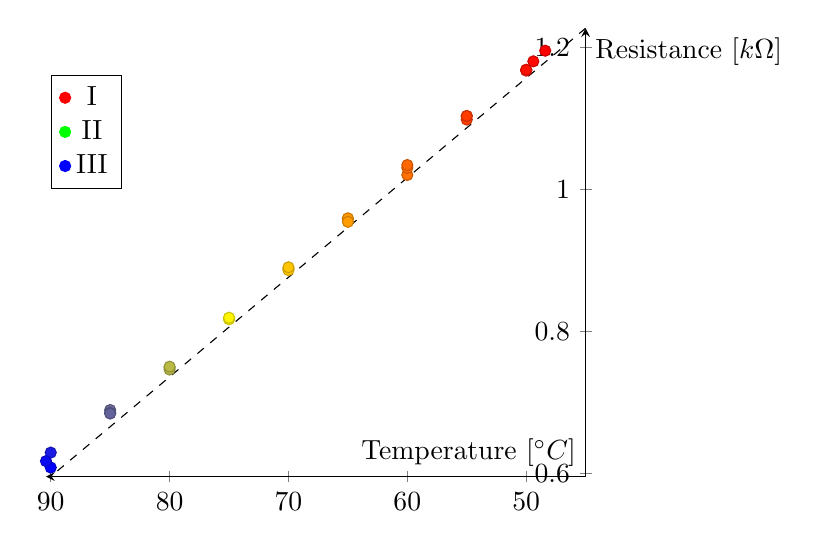
\begin{tikzpicture}
    \begin{axis}[
      axis lines=middle,
      x dir=reverse,
      legend style={
        at={(axis cs:90,1)},
        anchor=south west},
      xlabel=Temperature \lbrack$^{\circ}C$\rbrack,
      ylabel=Resistance \lbrack$k\Omega$\rbrack,
      ]
      \addplot[scatter,
      only marks,
      color=red,
      mark=*,
      ] coordinates {
        (90, 0.608)
        (85, 0.689)
        (80, 0.749)
        (75, 0.817)
        (70, 0.888)
        (65, 0.958)
        (60, 1.02)
        (55, 1.098)
        (50, 1.167)
      };
      \addlegendentry{\rom{1}}
      \addplot[scatter,
      only marks,
      color=green,
      mark=*,
      ] coordinates {
        (90, 0.629)
        (85, 0.685)
        (80, 0.746)
        (75, 0.817)
        (70, 0.886)
        (65, 0.959)
        (60, 1.03)
        (55, 1.103)
        (50, 1.168)
        (48.4, 1.195)
      };
      \addlegendentry{\rom{2}}
      \addplot[scatter,
      only marks,
      color=blue,
      mark=*,
      ] coordinates {
        (90.4, 0.617)
        (85, 0.684)
        (80, 0.75)
        (75, 0.819)
        (70, 0.89)
        (65, 0.954)
        (60, 1.034)
        (55, 1.103)
        (50, 1.168)
        (49.4, 1.18)
      };
      \addlegendentry{\rom{3}}
      \addplot[smooth, black, dashed][domain=45:90]{-0.01403*x+1.858};
    \end{axis}
  \end{tikzpicture}
  \label{fig:with}
  Fig.\ref{fig:with} Linear R-T 
\end{figure}
\section{Error Discussion}
\label{sec:error}
\section{Conclusion}
\end{document}
